\documentclass[../main.tex]{subfiles}

\begin{document}

SGX by itself, however, does not answer an imperative question: How do
you get the private key into the enclave in the first place? While the
key would be encrypted as it is used by an \textit{enclave program} in
RAM, it cannot be simply shipped as part of the binary. This is
because the binary is not encrypted. Yet, provisioning a web server
with a long-term private key for the purposes of SSL/TLS is currently
done by storing the private-key along with the executable on the
remote machine. This scheme, however, assumes a trusted
cloud-provider/OS. Therefore, to meet our above-stated goals,
this scheme is not viable.

Alternatively, we require a method that allows for the verification of
the identity and integrity of the server application, and then, upon
successful verification, we can send the long term private key to the
server in a secure fashion. Roughly, the requirements for this process
are as follows:
\begin{itemize}
  \item The mechanism allows the verification of the identity and
    integrity of the server application and the underlying TCB.  This is
    so that we can be sure the private-key is being sent to the same
    server we placed on the remote machine, and the software is being
    executed by trustworthy hardware.
  \item The mechanism allows us to setup a secure channel, ensuring that
    the only entities privy to the private key are the server
    application and the server administrator.
  \item The mechanism allows for the verification of the entity
    providing the private key. If this requirement were not in place,
    the mechanism could allow any arbitrary entity to authenticate with
    the server and provide their own private key. Observe that such an
    attack does not compromise the security of the long-term secret, but
    makes it possible to render the server useless (if the matching
    public certificate is not placed onto the server, verifying the
    server's hostname, then clients will reject connections to the
    server under the SSL/TLS protocol). % make this into a footnote?
\end{itemize}
The first and second requirement are met by a process called
inter-platform attestation, outlined by \Intel~
in~\cite{IntelCorporation2010} and summarized in the following
section\footnote{\Intel~ did not devise this mechanism, and it has been
used before in other Trusted Execution Environments (TEE) to
provision the TEE with highly sensitive secrets}.

\subsubsection{Inter-platform attestation and secret provisioning}

Inter-platform attestation is a mechanism that can be invoked by an
entity, referred to as the challenger, running on one platform to
verify an enclave running on another, remote, platform. This process
enables the challenger to verify the following about the remote
enclave:
\begin{enumerate}
  \item The contents of the enclave's pages (code, data, stack and heap)
    upon creation (after the ECREATE instruction completes)
  \item The identity of the entity that signed the enclave
  \item The trustworthiness of the underlying hardware
  \item Authenticity and integrity of any data generated by the enclave
    and sent as part of the attestation process. This allows us to
    satisfy the second requirement by generating an ephemeral key pair
    and binding it to the remote attestation process. This, therefore,
    allows the challenger to verify the integrity of the ephemeral
    public key and verify that it was generated by the server
    application.
\end{enumerate}
The steps involved in the attestation process are as follows
(illustrated in Figure~\ref{fig:attest}):

\begin{enumerate}
  \item The challenger invokes the remote attestation mechanism to
    verify the identity and integrity of the remote enclave
  \item The non-trusted part of the web server receives the challenge,
    passes it to the trusted portion of the web server along with
    the identity of the quoting enclave. The quoting enclave is a special
    enclave provided by Intel as part of the SGX platform to enable remote
    attestation by verifying the integrity of the underlying
    hardware. %refer readers to Intel white paper
  \item The enclave invokes EREPORT which is an SGX instruction that
    generates a REPORT structure to be provided to a \textit{local}
    enclave, the quoting enclave in this case.  This structure contains a
    hash of the contents of the enclave's pages upon ECREATE's termination
    (MRENCLAVE), a hash of the identity of the enclave's signer, a hash of
    any user-data, the ephemeral key in our case, generated by the
    enclave. The REPORT is signed by a MAC-key that can only be accessed
    by the CPU and the quoting enclave. The REPORT along with the
    ephemeral key is then sent to the non-trusted part of the application.
  \item The REPORT is sent to the quoting enclave where its integrity
    is verified by calculating the MAC across its contents.
  \item Assuming the REPORT is verified successfully, the quoting
    enclave generates a QUOTE structure that includes the REPORT structure
    and a signature across the QUOTE, generated using a key known as the
    EPID key. %add expansion of EPID
    The EPID key is a private key, unique
    to the CPU that is part of the platform, and verifies the firmware of
    the processor and its SGX capabilities.
  \item The QUOTE is sent along with the ephemeral key to the
    challenger
  \item The challenger verifies the QUOTE structure by using an EPID
    public certificate. If this is successful, the challenger is sure
    that this QUOTE came from a valid SGX CPU and can trust its
    authenticity. The challenger can then check the contents of the REPORT
    contained within the QUOTE to verify the identity of the remote
    enclave and the integrity of the ephemeral key received along with
    the QUOTE. The ephemeral key, if proven to be valid, can now be used
    to communicate with the remote enclave in a secure
    manner.\footnote{Verifying the certificate itself is conducted through
    contacting \Intel's attestation verification service}
\end{enumerate}
		
\begin{figure}[H]
  \centering
  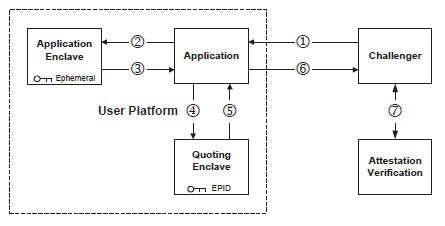
\includegraphics[scale=0.7]{attestation-sealing.jpg}
  \caption{Remote Attestation and Secret Provisioning}
  \label{fig:attest}
\end{figure}

\Intel has also added a construct that allows an \textit{enclave
program} to generate keys that can be used to encrypt sensitive data
and persisit it on disk. The only entities privy to the key are the
\textit{enclave program} and the CPU, therefore, only these two
entities can access the sealed data\footnote{This is not entirely
true, \Intel defined the EGETKEY instruction, the one that generates
the sealing keys such that it takes an argument of either MRENCLAVE or
MRSIGNER. If MRENCLAVE is used, then the sealing key generated is
unique to the invoking \textit{enclave program}. If MRSIGNER is used,
however, the sealing key generated is unique to all \textit{enclave
programs} signed by that entity}. This process, called sealing,
ensures that we execute the attestation process once, the first time
the \textit{enclave program} is launched, alleviating its cost.

However, the process outlined above takes no steps to verify the
challenging entity to the trusted component. In an effort to
authenticate the challenger, we utilize a combination of asymmetric
cryptography and SGX's guarantees.
% This needs more detail, but it contains the most important pieces of
% information
First, the server-administrator, before shipping the server program to
the cloud-provider, stores the public key for the challenger within
the text-area of the trusted component. The reason for this comes from
realizing that doing so binds the public key to the identity of the
trusted component, and as a result, the SGX-enabled CPU would not
start the trusted-component if the public key has been tampered
with. All that remains now is for challenger to sign the long term
private key with their own key, enabling the trusted-component to
verify it using the challenger's public-key that was shipped along
with the server-program.

\end{document}
